% =============================================================================
%  Cup Manipulator: Computed-Torque Controller, Direct-Drive & Cable-Spring
%  Dynamics Formulation
%  Files: robots/cup_manipulator_tendon.py  (ComputedTorqueController)
%         test_cup_manipulator_pendulam_with_spring_damper_pydrake_v2.py
%           (TendonSpringCompliance, ComputedTorqueSimulation)
% =============================================================================

\documentclass[11pt, a4paper]{article}

\usepackage[utf8]{inputenc}
\usepackage{amsmath, amssymb, bm}
\usepackage{geometry}
\usepackage{listings}
\usepackage{xcolor}
\usepackage{booktabs}
\usepackage{hyperref}
\usepackage{tikz}
\usetikzlibrary{arrows.meta, positioning, fit, shapes.geometric, calc}
\usepackage[backgroundcolor=blue!5, linecolor=blue!40, linewidth=1pt,
            innertopmargin=6pt, innerbottommargin=6pt,
            innerleftmargin=7pt, innerrightmargin=7pt]{mdframed}

\geometry{margin=2.2cm}

\lstset{
  language=Python,
  basicstyle=\ttfamily\small,
  keywordstyle=\color{blue!70!black},
  commentstyle=\color{gray},
  stringstyle=\color{orange!80!black},
  frame=single,
  breaklines=true,
  columns=fullflexible,
  backgroundcolor=\color{gray!8},
  xleftmargin=6pt, xrightmargin=6pt,
  aboveskip=4pt, belowskip=4pt,
  extendedchars=true,
  inputencoding=utf8,
  literate=
    {theta}{theta}5
    {tau}{tau}3
    {delta}{delta}5
    {omega}{omega}5
    {->}{->}2
    {>=}{>=}2
    {~=}{~=}2,
}

\newcommand{\rp}{r_p}
\newcommand{\bq}{\bm{q}}
\newcommand{\bqd}{\dot{\bm{q}}}
\newcommand{\bqdd}{\ddot{\bm{q}}}

% =============================================================================
\title{\textbf{Computed-Torque Controller \& Tendon Dynamics}\\
       \large Direct-Drive Joint~1 \;|\; Cable-Spring SEA Joint~2}
\date{March 2026}
\author{Isaac-sim robotics notes}
% =============================================================================

\begin{document}
\maketitle
\tableofcontents
\bigskip

% ---------------------------------------------------------------------------
\section{File Map}
% ---------------------------------------------------------------------------

\begin{center}
\begin{tabular}{ll}
\toprule
\textbf{File} & \textbf{Role} \\
\midrule
\texttt{robots/cup\_manipulator\_tendon.py}
  & \texttt{ComputedTorqueController} (Drake \texttt{LeafSystem}) \\
\texttt{test\_cup\_manipulator\_pendulam\_with\_} & \\
\quad\texttt{spring\_damper\_pydrake\_v2.py}
  & \texttt{TendonSpringCompliance} (SEA leaf system), \\
  & \texttt{ComputedTorqueSimulation} (diagram wiring) \\
\texttt{cable.py}
  & \texttt{PulleyBase}, pulley geometry, pitch-radius constant \\
\bottomrule
\end{tabular}
\end{center}

% ---------------------------------------------------------------------------
\section{Robot Overview: 2-DOF Planar Manipulator}
% ---------------------------------------------------------------------------

The cup manipulator has two revolute joints in the horizontal plane:

\begin{center}
\begin{tabular}{lll}
\toprule
\textbf{Joint} & \textbf{URDF name} & \textbf{Transmission} \\
\midrule
$q_1$ & \texttt{link1\_base}  & Direct-drive (no pulley in the torque path) \\
$q_2$ & \texttt{link2\_link1} & Cable \& HTD-5M belt via pulley of radius $\rp$ \\
\bottomrule
\end{tabular}
\end{center}

\noindent
Link lengths (URDF geometry):
\[
  L_1 = 342.47\,\text{mm}, \qquad L_2 = 190.00\,\text{mm}.
\]
HTD-5M 60-tooth pulley pitch radius:
\begin{equation}
  \rp = \frac{N \cdot p}{2\pi} = \frac{60 \times 5\,\text{mm}}{2\pi} \approx 47.75\,\text{mm}.
  \label{eq:pulley-radius}
\end{equation}

% ---------------------------------------------------------------------------
\section{Rigid-Body Dynamics (Plant)}
% ---------------------------------------------------------------------------

Drake models both joints as a single \texttt{MultibodyPlant}.
The standard manipulator equation is:
\begin{equation}
  M(\bq)\,\bqdd + C(\bq,\bqd)\,\bqd + g(\bq) = \bm{\tau}_{\text{plant}}
  \label{eq:eom}
\end{equation}
where $\bq = [q_1,\, q_2]^\top$, $M$ is the $2\times 2$ mass matrix,
$C\bqd$ collects Coriolis and centrifugal terms, and $g$ is the gravity vector.
$\bm{\tau}_{\text{plant}}$ is the torque vector that arrives at the plant's
actuation input port from either the controller (rigid tendon) or the SEA spring
(cable-spring mode).

\begin{lstlisting}
# Drake plant setup for both joints
plant = MultibodyPlant(time_step=0.002)   # dt = 2 ms
parser = Parser(plant, scene_graph)
manipulator.load_urdf_to_plant(plant, parser)
manipulator.weld_base_to_world(plant)
manipulator.add_end_effector_frame(plant)
manipulator.set_joint_properties(plant)   # viscous damping
manipulator.add_joint_actuators(plant)    # tau_link1_base, tau_link2_link1
plant.Finalize()
\end{lstlisting}

% ---------------------------------------------------------------------------
\section{Joint~1: Direct-Drive Dynamics}
% ---------------------------------------------------------------------------

Joint~1 is mechanically coupled directly to the motor shaft (no belt).
Newton's 2nd law on the motor+link1 inertia:
\begin{equation}
  \tau_1 = \tau_{1,\text{cmd}}
  \label{eq:j1-direct}
\end{equation}
The commanded torque reaches the joint without modification.
Drake's actuator for joint~1 is:

\begin{lstlisting}
# robots/cup_manipulator_tendon.py -- add_joint_actuators()
jt1 = manipulator.get_joint_by_name(plant, "link1_base")
act1 = plant.AddJointActuator("tau_link1_base", jt1, effort_limit)
# Optional motor model (AK80_8_KV60_Config etc.)
act1.set_default_rotor_inertia(rotor_inertia)
act1.set_default_gear_ratio(gear_ratio)
\end{lstlisting}

\noindent
When the motor model is configured, Drake automatically reflects the rotor
inertia and gear ratio into the plant dynamics, so $M(\bq)$ is augmented by
$N^2 I_\text{rotor}$ on the diagonal entry for $q_1$.

% ---------------------------------------------------------------------------
\section{Joint~2: Cable \& Spring (SEA) Dynamics}
% ---------------------------------------------------------------------------

\subsection{Rigid-Tendon Baseline (SEA Disabled)}

When $k_s = 0$ (default), the cable is modelled as perfectly rigid.
The commanded torque is delivered directly:
\begin{equation}
  \tau_{2,\text{plant}} = \tau_{2,\text{cmd}}.
  \label{eq:j2-rigid}
\end{equation}

\subsection{Series Elastic Actuator (SEA) Model}

When $k_s > 0$ a physical spring is inserted in the cable between the motor
pulley and joint~2.  The motor angle $\theta_m$ and joint angle $q_2$ are
now \emph{separate} degrees of freedom connected by the spring.

\paragraph{Cable stretch}
\begin{equation}
  \delta = \rp\,(\theta_m - q_2) \qquad [\text{m}]
  \label{eq:delta}
\end{equation}

\paragraph{Spring (cable) force}
\begin{equation}
  F_s = k_s\,\delta + b_s\,\dot\delta
      = k_s\,\rp\,(\theta_m - q_2) + b_s\,\rp\,(\dot\theta_m - \dot q_2)
      \qquad [\text{N}]
  \label{eq:Fs}
\end{equation}

\paragraph{Torque on joint~2 from spring}
\begin{equation}
  \tau_{2,\text{plant}} = F_s\,\rp
    = k_s\,\rp^2\,(\theta_m - q_2) + b_s\,\rp^2\,(\dot\theta_m - \dot q_2)
  \qquad [\text{Nm}]
  \label{eq:tau2-spring}
\end{equation}

\paragraph{Motor equation of motion}
Newton's 2nd law on the motor shaft (inertia $I_m$):
\begin{equation}
  I_m\,\ddot\theta_m = \tau_{2,\text{cmd}} - F_s\,\rp
    = \tau_{2,\text{cmd}} - k_s\,\rp^2\,(\theta_m - q_2)
      - b_s\,\rp^2\,(\dot\theta_m - \dot q_2)
  \label{eq:motor-eom}
\end{equation}

\paragraph{Full augmented system state}
Adding the SEA to the plant extends the state from
$\bm{x}_\text{plant} = [q_1, q_2, \dot q_1, \dot q_2]^\top$ to
\begin{equation}
  \bm{x} =
  \begin{bmatrix} q_1 \\ q_2 \\ \dot q_1 \\ \dot q_2 \\ \theta_m \\ \dot\theta_m \end{bmatrix},
  \quad
  \dot{\bm{x}} =
  \begin{bmatrix}
    \dot q_1 \\ \dot q_2 \\
    M^{-1}(\bm{\tau}_\text{plant} - C\bqd - g) \\
    \dot\theta_m \\
    \tfrac{1}{I_m}\bigl(\tau_{2,\text{cmd}} - F_s\,\rp\bigr)
  \end{bmatrix}
  \label{eq:augmented-state}
\end{equation}
where $\bm{\tau}_\text{plant} = [\tau_{1,\text{cmd}},\; F_s\,\rp]^\top$.

\begin{mdframed}
\textbf{Physical intuition.}
A weak spring ($k_s \approx 50$--$200\,\text{N/m}$) stretches significantly under
load: $\theta_m$ advances while $q_2$ lags.  This creates oscillatory, sluggish
joint-2 behaviour reminiscent of a tendon with finite stiffness.
A stiff spring ($k_s \gtrsim 5000\,\text{N/m}$) makes $\theta_m \approx q_2$,
recovering the rigid-tendon baseline.
\end{mdframed}

\subsection{TendonSpringCompliance LeafSystem}

The SEA is implemented as a Drake \texttt{LeafSystem} with two continuous
states $[\theta_m, \dot\theta_m]$:

\begin{lstlisting}
# test_cup_manipulator_pendulam_with_spring_damper_pydrake_v2.py

class TendonSpringCompliance(LeafSystem):
    # Ports
    #   In:  torque_cmd  [2]  -- [tau1_cmd, tau2_motor_cmd] from controller [Nm]
    #   In:  plant_state [n]  -- read q2, qdot2 from plant
    #   Out: torque_out  [2]  -- [tau1, tau2_spring] to plant actuation port [Nm]
    #   Out: spring_force[1]  -- F_s [N]  (logged separately)
    # Continuous state: [theta_m, theta_m_dot]

    def __init__(self, plant, manipulator,
                 k_s=500.0, b_s=2.0, I_m=5e-4):
        super().__init__()
        self._r_p = manipulator.PULLEY_RADIUS   # ~0.04775 m
        self._k_s = k_s;  self._b_s = b_s;  self._I_m = I_m
        self._plant_ctx = plant.CreateDefaultContext()  # private, for q2 reads
        nstate = plant.num_multibody_states()
        self._cmd_port   = self.DeclareVectorInputPort("torque_cmd",  2)
        self._state_port = self.DeclareVectorInputPort("plant_state", nstate)
        self.DeclareVectorOutputPort("torque_out",   2, self._calc_output)
        self.DeclareVectorOutputPort("spring_force", 1, self._calc_spring_force)
        self.DeclareContinuousState(2)           # [theta_m, theta_m_dot] continuous states
\end{lstlisting}

\subsubsection{Time Derivatives (Motor ODE)}

\begin{lstlisting}
    def _spring_force(self, context):
        # F_s = k_s * delta + b_s * delta_dot  [N]
        x = context.get_continuous_state_vector().CopyToVector()
        theta_m, theta_m_dot = x[0], x[1]
        q2, q2dot = self._read_joint2(context)  # from plant_state port
        r_p = self._r_p
        delta     = r_p * (theta_m - q2)           # cable stretch [m]
        delta_dot = r_p * (theta_m_dot - q2dot)    # rate  [m/s]
        return self._k_s * delta + self._b_s * delta_dot   # [N]

    def DoCalcTimeDerivatives(self, context, derivatives):
        tau_cmd = self._cmd_port.Eval(context)
        x = context.get_continuous_state_vector().CopyToVector()
        theta_m_dot = x[1]
        F_s = self._spring_force(context)
        # Motor EOM: I_m * theta_m_ddot = tau2_cmd - F_s * r_p
        theta_m_ddot = (tau_cmd[1] - F_s * self._r_p) / self._I_m
        derivatives.get_mutable_vector().SetAtIndex(0, theta_m_dot)
        derivatives.get_mutable_vector().SetAtIndex(1, theta_m_ddot)
\end{lstlisting}

\subsubsection{Output: Torque Delivered to Plant}

\begin{lstlisting}
    def _calc_output(self, context, output):
        tau_cmd = self._cmd_port.Eval(context)
        tau2_spring = self._spring_force(context) * self._r_p  # [Nm]
        # Joint 1: tau1 passes unmodified (direct-drive, no spring)
        # Joint 2: spring torque F_s*r_p delivered, NOT tau2_cmd directly
        output.SetFromVector(np.array([tau_cmd[0], tau2_spring]))
\end{lstlisting}

\subsubsection{Initialisation: Zero Spring Stretch at $t=0$}

To avoid an impulsive jerk at startup, the motor angle is seeded to match the
robot's initial joint-2 angle:

\begin{lstlisting}
    # In ComputedTorqueSimulation.initialize()
    if self.tendon_sys is not None:
        tendon_ctx = self.tendon_sys.GetMyMutableContextFromRoot(
            self.simulator.get_mutable_context()
        )
        # theta_m = q2 -- no initial spring stretch
        tendon_ctx.get_mutable_continuous_state_vector().SetAtIndex(0, q0[1])
        # theta_m_dot = 0
        tendon_ctx.get_mutable_continuous_state_vector().SetAtIndex(1, 0.0)
\end{lstlisting}

% ---------------------------------------------------------------------------
\section{Computed-Torque (Inverse-Dynamics) Controller}
% ---------------------------------------------------------------------------

\subsection{Feedback-Linearisation Law}

The computed-torque law cancels the nonlinear plant dynamics and imposes
desired linear 2nd-order error dynamics.

\paragraph{Step 1 — IK: Cartesian target $\to$ joint target}
\begin{equation}
  \bm{q}_\text{des}(t) = \text{IK}\bigl(\bm{p}_\text{ee,des}(t)\bigr)
  \label{eq:ik}
\end{equation}
Analytical 2R inverse kinematics; warm-started from the previous solution to
remain on the same elbow branch.

\paragraph{Step 2 — Reference feedforward in joint space}

The 2R Jacobian at $\bm{q}_\text{des}$:
\begin{equation}
  J(\bm{q}) =
  \begin{bmatrix}
    -L_1\sin q_1 - L_2\sin(q_1+q_2) & -L_2\sin(q_1+q_2) \\
     L_1\cos q_1 + L_2\cos(q_1+q_2) &  L_2\cos(q_1+q_2)
  \end{bmatrix}
  \label{eq:jacobian}
\end{equation}
Reference joint velocity and acceleration via pseudoinverse:
\begin{equation}
  \dot{\bm{q}}_\text{ref} = J^+ \dot{\bm{p}}_\text{ref}, \qquad
  \ddot{\bm{q}}_\text{ref} \approx J^+ \ddot{\bm{p}}_\text{ref}
  \quad (\dot{J}\dot{\bm{q}}\text{ bias dropped})
  \label{eq:jac-inv}
\end{equation}

\paragraph{Step 3 — Desired joint acceleration (PD + feedforward)}
\begin{equation}
  \boxed{\bm{a}_\text{des} = \ddot{\bm{q}}_\text{ref}
    + K_p\,(\bm{q}_\text{des} - \bm{q})
    + K_d\,(\dot{\bm{q}}_\text{ref} - \dot{\bm{q}})}
  \label{eq:a-des}
\end{equation}

\paragraph{Step 4 — Inverse dynamics: acceleration $\to$ torque}
\begin{equation}
  \bm{\tau} = M(\bm{q})\,\bm{a}_\text{des} + C(\bm{q},\dot{\bm{q}})\,\dot{\bm{q}} + g(\bm{q})
  \label{eq:idyn}
\end{equation}
Drake evaluates \eqref{eq:idyn} via \texttt{CalcInverseDynamics} (internally
uses the equation $\bm{\tau} = M\,\dot{v} + \text{bias}$, gravity included):

\begin{lstlisting}
# robots/cup_manipulator_tendon.py -- ComputedTorqueController._solve()

# Map a_des from user-order [q1,q2] to Drake nv-vector
a_des_drake = np.zeros(nv)
a_des_drake[self._v_idx[0]] = a_des_user[0]
a_des_drake[self._v_idx[1]] = a_des_user[1]

# Inverse dynamics: tau = M(q)*a_des + C(q,v)*v + g(q)
self._forces.SetZero()           # no additional external forces
tau_full = self._plant.CalcInverseDynamics(
    self._plant_ctx, a_des_drake, self._forces
)
tau1 = float(tau_full[self._v_idx[0]])
tau2 = float(tau_full[self._v_idx[1]])
\end{lstlisting}

\subsection{Closed-Loop Error Dynamics}

Substituting \eqref{eq:idyn} into \eqref{eq:eom} gives decoupled linear
2nd-order systems for each joint:
\begin{equation}
  \ddot{e}_i + K_d\,\dot{e}_i + K_p\,e_i = 0, \qquad
  e_i = q_{i,\text{des}} - q_i
  \label{eq:closed-loop}
\end{equation}
with complex poles at:
\begin{equation}
  s = -\zeta\omega_n \pm \omega_n\sqrt{\zeta^2 - 1}, \qquad
  \omega_n = \sqrt{K_p}, \quad
  \zeta = \frac{K_d}{2\sqrt{K_p}}
  \label{eq:poles}
\end{equation}
Default gains: $K_p = 400\,\text{s}^{-2}$, $K_d = 40\,\text{s}^{-1}$
$\Rightarrow \omega_n = 20\,\text{rad/s}$, $\zeta = 1$ (critically damped).

\begin{lstlisting}
# Feedforward + PD law -- ComputedTorqueController._solve()
ee_vel_ref = self._vel_port.Eval(context)   # EE vel ref  [m/s]
ee_acc_ref = self._acc_port.Eval(context)   # EE acc ref  [m/s^2]
q1d, q2d = q_des
s1  = np.sin(q1d);          c1  = np.cos(q1d)
s12 = np.sin(q1d + q2d);    c12 = np.cos(q1d + q2d)
J = np.array([
    [-self._L1 * s1 - self._L2 * s12, -self._L2 * s12],
    [ self._L1 * c1 + self._L2 * c12,  self._L2 * c12],
])
J_inv      = np.linalg.pinv(J)
q_dot_ref  = J_inv @ ee_vel_ref          # joint vel ref [rad/s]
q_ddot_ref = J_inv @ ee_acc_ref          # joint acc ref [rad/s^2]

# Full CT: feedforward + PD feedback
a_des_user = (q_ddot_ref
              + self._Kp * (q_des - q)
              + self._Kd * (q_dot_ref - q_dot))
\end{lstlisting}

\subsection{Joint-2 Cable Tension Decomposition}

Because cables can only pull ($T \ge 0$), the signed torque $\tau_2$ is
resolved into two non-negative tensions (retracting and extending cables):
\begin{equation}
  F_\text{net} = \frac{\tau_2}{\rp}, \qquad
  T_\text{green} = \max(F_\text{net},\;0), \qquad
  T_\text{red}   = \max(-F_\text{net},\;0)
  \label{eq:tension-decomp}
\end{equation}
\begin{equation}
  \tau_{2,\text{cmd}} = (T_\text{green} - T_\text{red})\,\rp = \tau_2
\end{equation}

\begin{lstlisting}
# Cable tension decomposition -- ComputedTorqueController._solve()
F_net   = tau2 / self._r_p                  # net cable force [N]
T_green = max(F_net,  0.0)                  # retracting side (>=0)
T_red   = max(-F_net, 0.0)                  # extending side  (>=0)
tau2_cmd = (T_green - T_red) * self._r_p    # = tau2; logged separately
tau_clip = np.clip([tau1, tau2_cmd], -self._tau_max, self._tau_max)
\end{lstlisting}

% ---------------------------------------------------------------------------
\section{Diagram: Controller + SEA Wiring}
% ---------------------------------------------------------------------------

\subsection{Block Diagram}

\begin{center}
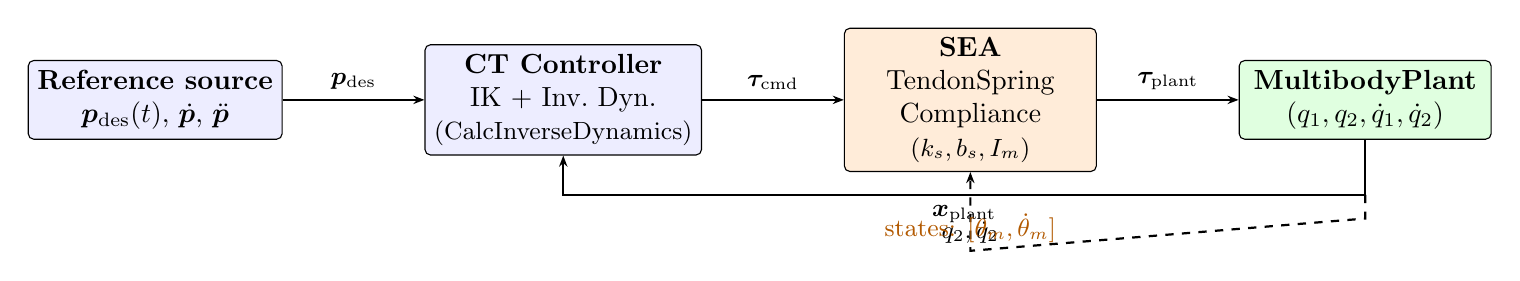
\begin{tikzpicture}[
  node distance = 9mm and 18mm,
  block/.style  = {draw, rectangle, rounded corners=2pt,
                   minimum width=3.2cm, minimum height=1.0cm,
                   align=center, fill=blue!7},
  sea/.style    = {draw, rectangle, rounded corners=2pt,
                   minimum width=3.2cm, minimum height=1.0cm,
                   align=center, fill=orange!15},
  plant/.style  = {draw, rectangle, rounded corners=2pt,
                   minimum width=3.2cm, minimum height=1.0cm,
                   align=center, fill=green!12},
  arr/.style    = {-{Stealth[length=4pt]}, thick},
]

\node[block]  (ref)  {\textbf{Reference source}\\$\bm{p}_\text{des}(t)$, $\dot{\bm{p}}$, $\ddot{\bm{p}}$};
\node[block, right=of ref]  (ct)   {\textbf{CT Controller}\\IK + Inv.\ Dyn.\\\small(CalcInverseDynamics)};
\node[sea,   right=of ct]   (sea)  {\textbf{SEA}\\TendonSpring\\Compliance\\\small$(k_s, b_s, I_m)$};
\node[plant, right=of sea]  (pl)   {\textbf{MultibodyPlant}\\$(q_1, q_2, \dot q_1, \dot q_2)$};

\draw[arr] (ref) -- node[above]{\small$\bm{p}_\text{des}$} (ct);
\draw[arr] (ct)  -- node[above]{\small$\bm{\tau}_\text{cmd}$} (sea);
\draw[arr] (sea) -- node[above]{\small$\bm{\tau}_\text{plant}$} (pl);

% Feedback: plant_state -> CT controller
\draw[arr] (pl.south) -- ++(0,-0.7) -| node[pos=0.25, below]{\small$\bm{x}_\text{plant}$} (ct.south);

% plant_state -> SEA (for q2 reading)
\draw[arr, dashed] (pl.south) ++(0,-0.7) -- ++(0,-0.3)
  -- ($(sea.south)+(0,-1.0)$)
  -- node[below]{\small$q_2,\dot q_2$} (sea.south);

% SEA internal state annotation
\node[below=4mm of sea, align=center, font=\small, text=orange!70!black]
  {states: $[\theta_m, \dot\theta_m]$};

\end{tikzpicture}
\end{center}

\noindent
Dashed arrow: the \texttt{plant\_state} port is connected to the SEA to read
$q_2, \dot q_2$ at each integration step.  When the SEA is disabled
($k_s = 0$), the direct wire $\bm{\tau}_\text{cmd} \to$ plant is used instead.

\subsection{Drake Diagram Wiring Code}

\begin{lstlisting}
# ComputedTorqueSimulation.connect_and_build()

# Controller receives: EE reference + plant state
builder.Connect(ee_ref.get_output_port(),
                ik_system.GetInputPort("desired_ee_pos"))
builder.Connect(ee_vel_src.get_output_port(),
                ik_system.GetInputPort("ee_vel_ref"))
builder.Connect(ee_acc_src.get_output_port(),
                ik_system.GetInputPort("ee_acc_ref"))
builder.Connect(plant.get_state_output_port(),
                ik_system.GetInputPort("plant_state"))

if tendon_stiffness > 0:                         # SEA enabled
    sea = builder.AddSystem(TendonSpringCompliance(
        plant, manipulator,
        k_s=tendon_stiffness,
        b_s=tendon_damping,
        I_m=tendon_motor_inertia,
    ))
    # Controller -- SEA -- plant
    builder.Connect(ik_system.GetOutputPort("actuation"),
                    sea.GetInputPort("torque_cmd"))
    builder.Connect(plant.get_state_output_port(),
                    sea.GetInputPort("plant_state"))   # feeds q2, qdot2
    builder.Connect(sea.GetOutputPort("torque_out"),
                    plant.get_actuation_input_port())
else:                                            # rigid tendon
    builder.Connect(ik_system.GetOutputPort("actuation"),
                    plant.get_actuation_input_port())
\end{lstlisting}

% ---------------------------------------------------------------------------
\section{Gain Selection Guide}
% ---------------------------------------------------------------------------

\begin{center}
\begin{tabular}{ll p{7.5cm}}
\toprule
\textbf{Parameter} & \textbf{Default} & \textbf{Interpretation / effect} \\
\midrule
$K_p$ & 400 s$^{-2}$ & Natural frequency $\omega_n = \sqrt{K_p}$.
                        Larger $K_p$ → faster convergence; too large → instability
                        with SEA. \\
$K_d$ & 40 s$^{-1}$  & Damping ratio $\zeta = K_d / (2\omega_n)$.
                        Default $\zeta = 1$ (critically damped, no overshoot). \\
$k_s$ & 0 N/m        & SEA spring stiffness.  $k_s = 0$ → rigid tendon.
                        $k_s = 100$ → noticeably laggy J2.
                        $k_s = 5000$ → quasi-rigid. \\
$b_s$ & 2 N·s/m      & SEA cable viscous damping.  Increases spring damping ratio. \\
$I_m$ & $5{\times}10^{-4}$ kg·m$^2$
                      & Motor rotor inertia.  Larger $I_m$ → longer oscillation
                        period (slower motor response). \\
\bottomrule
\end{tabular}
\end{center}

% ---------------------------------------------------------------------------
\section{CLI Usage}
% ---------------------------------------------------------------------------

\begin{lstlisting}[language=bash]
# Rigid tendon (default)
python test_cup_manipulator_pendulam_with_spring_damper_pydrake_v2.py \
    --mode computed-torque --duration 10

# Weak SEA (slug-like J2, clear lag)
python ... --mode computed-torque \
    --tendon-stiffness 100 --tendon-damping 2 --tendon-motor-inertia 5e-4

# Stiff SEA (near-rigid, small residual oscillation)
python ... --mode computed-torque \
    --tendon-stiffness 5000 --tendon-damping 5 --tendon-motor-inertia 5e-4

# Custom CT gains (higher bandwidth)
python ... --mode computed-torque --ct-kp 900 --ct-kd 60
\end{lstlisting}

\end{document}
